\let\negmedspace\undefined
\let\negthickspace\undefined
\documentclass[journal,12pt,onecolumn]{IEEEtran}
\usepackage{cite}
\usepackage{amsmath,amssymb,amsfonts,amsthm}
\usepackage{algorithmic}
\usepackage{graphicx}
\graphicspath{{Figs/}}
\usepackage{textcomp}
\usepackage{xcolor}
\usepackage{txfonts}
\usepackage{listings}
\usepackage{enumitem}
\usepackage{mathtools}
\usepackage{gensymb}
\usepackage{comment}
\usepackage{caption}
\usepackage[breaklinks=true]{hyperref}
\usepackage{tkz-euclide} 
\usepackage{listings}
\usepackage{gvv}                                        
%\def\inputGnumericTable{}                                 
\usepackage[latin1]{inputenc}     
\usepackage{xparse}
\usepackage{color}                                            
\usepackage{array}                                            
\usepackage{longtable}                                       
\usepackage{calc}                                             
\usepackage{multirow}
\usepackage{multicol}
\usepackage{hhline}                                           
\usepackage{ifthen}                                           
\usepackage{lscape}
\usepackage{tabularx}
\usepackage{array}
\usepackage{float}
%\newtheorem{theorem}{Theorem}[section]
%\newtheorem{theorem}{Theorem}[section]
%\newtheorem{problem}{Problem}
%\newtheorem{proposition}{Proposition}[section]
%\newtheorem{lemma}{Lemma}[section]
%\newtheorem{corollary}[theorem]{Corollary}
%\newtheorem{example}{Example}[section]
%\newtheorem{definition}[problem]{Definition}

\begin{document}

\title{1.11.4}
\author{AI25BTECH11002 - Ayush Sunil Labhade}
{\let\newpage\relax\maketitle}
%\renewcommand{\thefigure}{\theenumi}
%\renewcommand{\thetable}{\theenumi}
		\textbf{Question}:\newline

		A vector of magnitude 9 units in the direction of the vector $-2\hat{\imath}-\hat{\jmath}+2\hat{k}$

		\textbf{Solution:}
		The vector with magnitude 9 in the same direction would be: 
		\begin{align}
			\|c\myvec{-2 & -1 & 2}^T\| = 9
		\end{align}
		\begin{align}
		\therefore |c|=3
		\end{align}
		Thus, the vector is:
		\begin{align}
			\myvec{-6 \\ -3\\6}
		\end{align}
		Graph:
\begin{figure}[H]
	\centering
	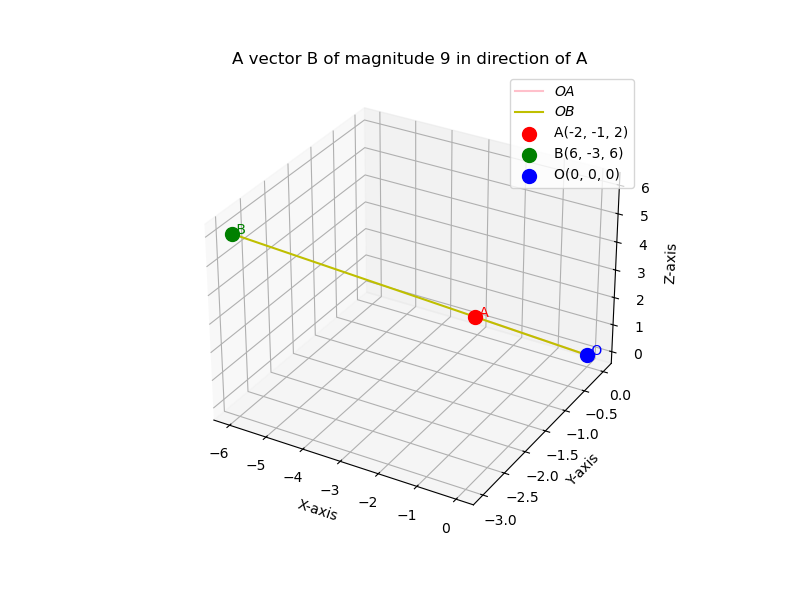
\includegraphics[scale=0.5]{plot}
	\caption*{}
	\label{fig}
\end{figure}
\end{document}
